\documentclass[french]{article}
\usepackage[utf8x]{inputenc}
\usepackage[T1]{fontenc}
\usepackage{babel}
\usepackage{lmodern}
\usepackage[top=2cm,bottom=2cm,left=3cm,right=3cm]{geometry}
\usepackage{microtype}
\usepackage{mathtools, amssymb, amsthm}
\usepackage{dsfont}
\usepackage{mdframed}
\usepackage{hyperref}
\usepackage{graphicx}
\usepackage{xcolor}
\usepackage{mathrsfs}
\usepackage{wrapfig}
\usepackage{stmaryrd}

\newtheorem{prop}{Proposition}[section]
\newtheorem{theorem}{Théorème}
\newtheorem{definition}{Définition}[section]
\newtheorem*{remark}{Remarque}
\newtheorem*{lemma}{Lemme}
\newtheorem*{corollary}{Corollaire}
\newtheorem*{mth}{Méthode}
\newmdtheoremenv{thm}{Théorème}
\newtheorem{exo}{Exercice}
\newtheorem{exemple}{Exemple}


\newcommand*{\TakeFourierOrnament}[1]{{%
\fontencoding{U}\fontfamily{futs}selectfont\char#1}}
\newcommand*{\danger}{\TakeFourierOrnament{66}}

\newcommand{\lesss}{\rotatebox[origin=c]{90}{$\land$}}
\newcommand{\less}{\ \lesss\ }

\newcommand{\biggg}{\rotatebox[origin=c]{90}{$\lor$}}
\newcommand{\bg}{\ \biggg\ }

\title{\bsc{Géométrie différentielle}}
\date{2023-2024}

\begin{document}

\maketitle

\tableofcontents

\section{Fonctions continues}


$U \subseteq \mathbb{R}^n$ ouvert.

$f:
  \begin{array}{lll}
  U & \longrightarrow & \mathbb{R} \\
  (x_1, \dots, x_n) & \longmapsto f(x_1, \dots, x_n)
  \end{array}$ application.

$f$ est continue en $x_0$ dans $U$ si $$\forall \varepsilon \bg 0, \exists \delta  \bg 0, \forall x \in U, \Vert x-x_0 \Vert \less \delta \to \lvert f(x)-f(x_0) \rvert \less \varepsilon,  $$

avec $\Vert y \Vert = \sqrt{ y_1 ^2 + \dots + y_n ^2 }  $.

On dit que $f$ est une application continue quand $f$ est continue en $x \in U$ pour tout $x \in U$.

\begin{prop}
  $f$ est continue si et seulement si pour tout intervalle ouvert $J \subseteq \mathbb{R}$, $f ^{-1} (J)$ est ouvert, avec $f ^{-1} (J) := \{ x \in U \mid f(x) \in J \} $.
\end{prop}

\begin{proof}
  \begin{enumerate}
    \item \emph{Si $f$ est continue, alors $ \forall J \subset \mathbb{R}$ intervalle ouvert, $f ^{-1} (J)$ est ouvert.}

    Il faut montrer que $\forall x_0 \in f ^{-1} (J)$, il existe $r \bg 0$ tel que $B(x_0, r) \subset f ^{-1} (J)$.

    \begin{figure}[h!]
      \centering
      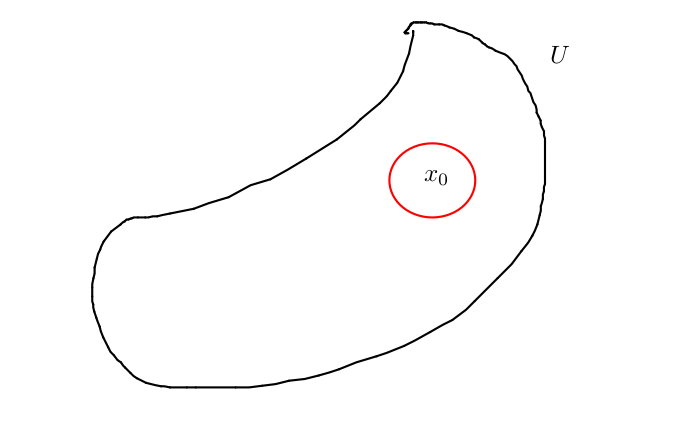
\includegraphics[scale=0.3]{figures/recip_ouvert.png}
      \caption{Illustration}
      \label{}
    \end{figure}

    $J = (a,b)$.

    $x_0 \in f ^{-1} (J) \implies f(x_0) \in J \implies a \less f(x_0) \less b \implies \exists \varepsilon  \bg 0 \text{ tel que } $

    $$ a \less f(x_0) - \varepsilon \less f(x_0) \less f(x_0) + \varepsilon \less b.$$

    On peut choisir $\varepsilon = \min \{ \frac{b-f(x_0)}{2}, \frac{f(x_0)-a}{2} \} $.

    \begin{figure}[h!]
      \centering
      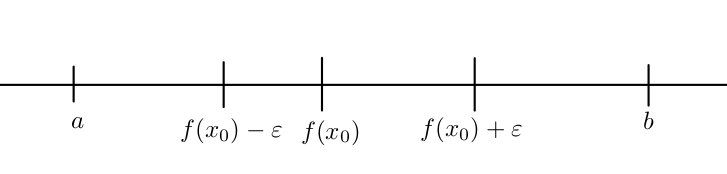
\includegraphics[scale=0.3]{figures/demo_prop_1.png}
      \caption{On choisit $\varepsilon $ de cette sorte}
      \label{}
    \end{figure}

    Donc il y a $\delta \bg 0$ tel que

    \begin{gather*}
      \Vert x-x_0 \Vert \less \delta  \implies \lvert f(x)- f(x_0) \rvert \less \varepsilon \\
      \implies - \varepsilon \less f(x) -f(x_0) \less \varepsilon \\
      \implies f(x_0) - \varepsilon \less f(x) \less f(x_0)+ \varepsilon \implies a \less f(x) \less b \\
      \implies f(x) \in J \implies x \in f ^{-1} (J).
    \end{gather*}

    Choisissons $r := \delta $

    $x \in B(x_0, r) \implies \Vert x-x_0 \Vert \less r=\delta  $.

    On a démontré que avec ce choix de $\delta $ on a $x \in f ^{-1} (J) \implies B(x_0, r) \subset f ^{-1} (J)$.

    \item \emph{Si $f ^{-1} (J)$ ouvert pour tout intervalle $J \subset \mathbb{R}$, alors $f$ est continue.}

    Fixons $x_0 \in U : \varepsilon \bg 0$ est donné.

    On met $J = (f(x_0) - \varepsilon , f(x_0)+ \varepsilon ) \neq \emptyset$.

    Par l'hypothèse, $f ^{-1} (J)$ est ouvert, donc $\exists r \bg 0, B(x_0, r) \subset f ^{-1} (J)$.

    On met $\delta := r$.

    \begin{gather*}
      \Vert x-x_0 \Vert \less \delta \implies x \in B(x_0, \delta ) = B(x_0, r)\\
      \implies x \in f ^{-1} (J) \implies f(x) \in J \\
      \implies f(x_0) - \varepsilon \less f(x) \less f(x_0) + \varepsilon \implies - \varepsilon \less f(x) - f(x_0) \less \varepsilon \\
      \implies \lvert f(x) - f(x_0) \rvert \less \varepsilon .
    \end{gather*}
  \end{enumerate}
\end{proof}

On peut aussi généraliser ces définitions et la proposition aux cas où $f: U \to \mathbb{R}^m$ est une application de $U$ dans $\mathbb{R}^m$, avec

$$ f(x_1, \dots, x_n) = (f_1(x_1, \dots, x_n), \dots, f_m(x_1, \dots, x_m)).$$

\paragraph{Exemple}

$f(x_1, x_2) = (x_1 ^2+ 3 \cos(x_2) e^{x_1-x_2} )$, $n=2, m=2, U = \mathbb{R}^2$.

\begin{definition}
  $f$ est continue en $x_0 \in U$ si

  $$ \forall \varepsilon  \bg 0, \exists \delta  \bg 0, \forall x \in U, \Vert x-x_0 \Vert \less \delta \implies \Vert f(x)-f(x_0) \Vert \less \varepsilon, $$

  avec   $\Vert f(x)-f(x_0) \Vert = \sqrt{ (f_1(x)-f_1(x_0)) ^2 + \dots + (f_m(x)-f_m(x_0)) ^2 } $.
\end{definition}

\begin{definition}
  $f : U \to \mathbb{R}^m$ est continue quand $f$ est continue en $x, \forall x \in U$.
\end{definition}

\begin{prop} \label{continue}
  Les 3 conditions suivantes sont équivalentes.

  \begin{enumerate}
    \item $f : U \to \mathbb{R}^m$ est continue ;
    \item $\forall j \in \{ 1, \dots, m \} $, $f_j$ est continue ;
    \item $\forall V \subseteq \mathbb{R}^m$ ensemble ouvert, $f  ^{-1} (V)$ est ouvert.
  \end{enumerate}
\end{prop}

\begin{figure}[h!]
  \centering
  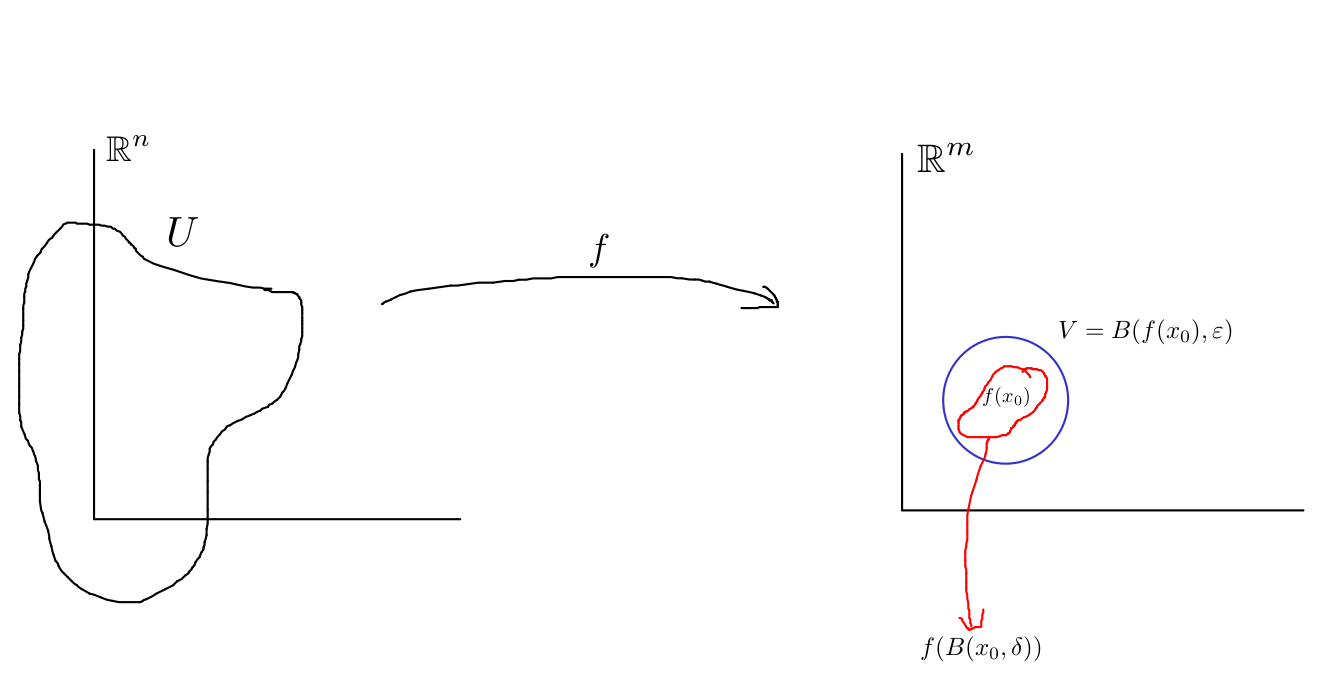
\includegraphics[scale=0.2]{figures/boule_continue.png}
  \caption{Illustration pour \ref{continue}}
  \label{}
\end{figure}



\section{Dérivée, dérivée partielle, différentielle}

$ f : U \to \mathbb{R}$.

$x \in U$ fixé.

La dérivée partielle $\frac{\partial f }{\partial x_i} $, pour $ i \in \{ 1, \dots, n \} $ et $x = (x_1, \dots, x_n)$ est définie par

\begin{gather*}
  \frac{\partial f }{\partial x_i} (x_1, \dots, x_n) := \lim_{h \to 0} \frac{f(x_1, \dots, x_i + h, \dots, x_n)}{h}
\end{gather*}

si la limite existe.

Si $e_i \in \mathbb{R}^n$ est le vecteur $e_i = (0,0,  \dots, 0, \overbrace{1}^{i\text{-ème}}, 0, \dots, 0)$ (tel que $\{ e_1, \dots, e_n \} $ est la base standart de l'espace linéaire $\mathbb{R}^n$), on a

\begin{gather*}
  \frac{\partial f }{\partial x_i }(x) := \lim_{h \to 0} \frac{f(x+h e_i)}{h}  .
\end{gather*}

On peut aussi calculer les dérivées partielles de $\frac{\partial f }{\partial x_i} $. En général, pour tout $k \geq 1$, $$ \frac{\partial ^{k} f }{\partial x_k \partial x _{k-1} \dots \partial x_2 \partial x_1 }  = \frac{\partial  }{\partial x_k } \left(\frac{\partial  }{\partial x _{k-1} } \dots \left(\frac{\partial f }{\partial x_1} \right) \right) .$$

$i_1 \in \{ 1, \dots, n \}, \dots, i_k \in \{ 1, \dots, n \} $.

Pour $k=1$, il y a $n$ dérivées partielles.

Pour $k=2, i_1 \longrightarrow$ $n$ choix de $\{ 1, \dots, n \} $.

$i_2 \longrightarrow $ $n$ choix.

Donc il y a $n ^2$ choix.

En général, il y a $n ^{k}$ dérivées partielles différentes de l'ordre $k$.

\begin{definition}
  $r \in \mathbb{N}$.

  On dit que $f : U \to \mathbb{R}$ est une application de classe $\mathcal{C}^r$  ou tout simplement $f$ est $\mathcal{C}^r$ quand

  \begin{enumerate}
    \item Si $r=0$, $f$ est continue.
    \item Si $r \geq 1$, $f$ est continue et les dérivées partielles d'ordre $k$ existent partout dans $U$ et elles sont toutes les applications continues dans $U$ et ceci pour tout $ 1 \leq k \leq r$.
    \item Pour $f : U \to \mathbb{R}^m$, une application, on dit que $f$ est $\mathcal{C}^r$ si $\forall j \in \{ 1, \dots, m \} $, $f_j$ est une application $\mathcal{C}^r$, avec $f = (f_1, \dots, f_m)$.

    On dit que $f$ est $\mathcal{C}^\infty$ quand $\forall r \in \mathbb{N}$, $f$ est $\mathcal{C}^r$.
  \end{enumerate}
\end{definition}

\subsection{Différentiabilité des fonctions multi-variables}

$U \subseteq \mathbb{R}^n$ ouvert, $f : U \to \mathbb{R}^n$, $x=(x_1, \dots, x_n) \in U$, $f = (f_1, \dots, f_m)$.

On dit que $f$ est différentiable à $x \in U$ quand il existe une application linéaire $L : \mathbb{R}^n \to \mathbb{R}^m$ telle que

\begin{gather*}
  \forall \varepsilon \bg 0, \exists \delta  \bg 0 \text{ si } \Vert h \Vert \less \delta \text{ et } x+h \in U, \text{ alors } \Vert f(x+h) - (f(x)+L(h)) \Vert \less \varepsilon \Vert h \Vert .
\end{gather*}

\begin{figure}[h!]
  \centering
  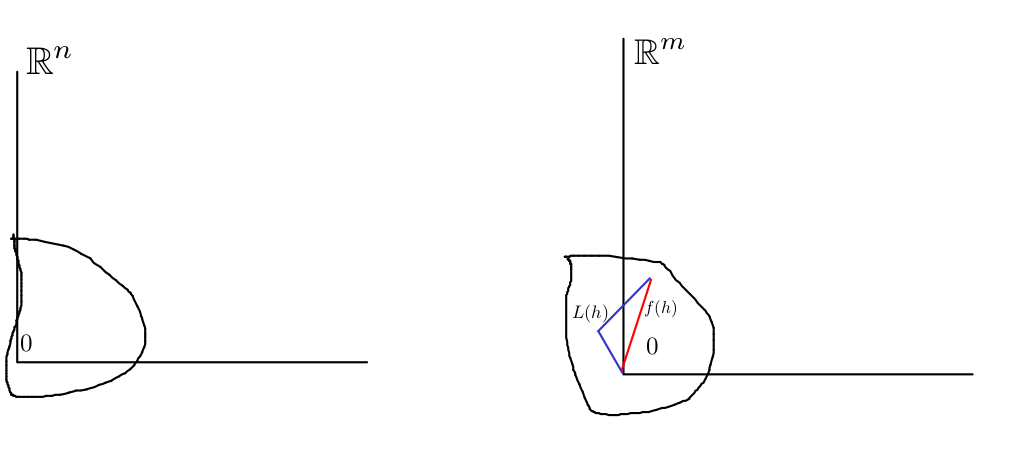
\includegraphics[scale=0.3]{figures/diff.png}
  \caption{Exemple illustratif avec $x=0, f(0) = 0$}
  \label{}
\end{figure}

$f$ différentiable en 0 si $\forall \varepsilon  \bg 0$, $\exists \delta \bg 0, \Vert h \Vert \less \delta \implies \Vert f(h) - L(h) \Vert \less \varepsilon \Vert h \Vert  $.

\begin{prop}
  $n=1, m=1, f : I \to \mathbb{R}$ est différentiable selon la définition donnée sur un point $x \in I$ si et seulement si $f'(x)$ existe.
\end{prop}

\begin{proof}

  \

  \begin{enumerate}
    \item \emph{Sens direct : $f$ différentiable en $x \in I$ $\implies f'(x)$ existe.}

    $\exists L : \mathbb{R} \to \mathbb{R}$ telle que

    $$ \forall \varepsilon \bg 0, \exists \delta \bg 0, \Vert h \Vert \less \delta , x+h \in I \implies \Vert f(x+h) - f(x) -L(h) \Vert \less \varepsilon \Vert h \Vert.$$

    $L(h) = ah$ pour un $a \in \mathbb{R}$ quelconque mais fixé.

    $a$ est la pente ou le coefficient directeur.

    Prenons $a$   la pente du graphe de $L$ (comme $L$ linéaire, $\exists a \in \mathbb{R}$ tel que $\forall h \in \mathbb{R}, L(h) = ah$).

    On obtient

    $$ \forall \varepsilon \bg 0, \exists \delta \bg 0, \lvert h \rvert \less \delta , x+h \in I \implies \lvert f(x+h) -f(x)-ah \rvert \leq \varepsilon \lvert h \rvert.$$

    On divise par $\lvert h \rvert \neq 0$ pour obtenir

    \begin{gather*}
      \left\lvert \frac{f(x+h)-f(x)}{h} - \frac{ah}{h} \right\rvert \leq \varepsilon.
    \end{gather*}

    \begin{gather*}
      \forall \varepsilon  \bg 0, \exists \delta  \bg 0 \text{ tel que } \lvert h \rvert \less \delta , h+x \in I, \text{ alors } \left\lvert \frac{f(x+h)-f(x)}{h}-a \right\rvert \leq \varepsilon,
    \end{gather*}

    c'est à dire

    \begin{gather*}
      \lim_{h \to 0} \frac{f(x+h)-f(x)}{h} = a.
    \end{gather*}

    Donc $f'(x)$ existe et $f'(x) = a$.

    \item \emph{Sens réciproque : $f'(x)$ existe $\implies f$ différentiable.}

    Si $f'(x)$ existe, on met $a :=f'(x)$.

    On définit $L(h) =ah$. On sait que

    $$ \lim_{h \to 0} \frac{f(x+h)-f(x)}{h} = f'(x) = a.$$

    Donc

    \begin{gather*}
      \forall \varepsilon \bg 0, \exists \delta  \bg 0, \lvert h \rvert \less \delta \implies \left\lvert \frac{f(x+h)-f(x)}{h} -a \right\rvert \leq \varepsilon  \\
      \implies \lvert f(x+h) -f(x) -ah \rvert \leq \varepsilon \lvert h \rvert \\
      \implies \forall h, \lvert h \rvert \less \delta, \text{ on a } \lvert f(x+h) - f(x) -ah \rvert \leq \varepsilon \lvert h \rvert.
    \end{gather*}

    $f$ est différentiable selon notre définition avec $L(h) =ah$.
  \end{enumerate}
\end{proof}


On suppose maintenant que $f:U \to \mathbb{R}^m, U \subseteq \mathbb{R}^n$.

Pour $x \in U$, $f$ différentiable en $x$ si $\exists L : \mathbb{R}^n \to \mathbb{R}^m$ linéaire telle que

\begin{gather*}
  \forall \varepsilon  \bg 0, \exists \delta  \bg 0, \forall h \in \mathbb{R}^n, \Vert h \Vert \less \delta, x+h \in U \implies \Vert f(x+h) -f(x)-L(h) \Vert \leq \varepsilon \Vert h \Vert.
\end{gather*}

On note $\mathscr{L}(\mathbb{R}^n, \mathbb{R}^m) = \{  T: \mathbb{R}^n \to \mathbb{R}^m \mid T \text{ est linéaire }   \} $.

On écrit dans ce cas là que $Df(x) = L \in \mathscr{L}(\mathbb{R}^n, \mathbb{R}^m)  $.

En particulier, si $f$ est différentiable pour tout $x \in U$, on obtient une application $$Df : U \to \mathscr{L}(\mathbb{R}^n, \mathbb{R}^m). $$

\subparagraph{Rappel} Chaque transformation linéaire est uniquement représentée par une matrice au cas où les bases des espaces de départ et d'arrivée sont fixées.

Si on choisit les bases standart $\alpha = \{ e_1, \dots, e_n \} $ pour $ \mathbb{R}^n$ et $ \beta = \{ e_1, \dots, e_m \} \in \mathbb{R}^m $, $T \in \mathscr{L}(\mathbb{R}^n, \mathbb{R}^m) $.

$$ [T] _{\beta } ^{\alpha} := A = [A _{ij}] _{m \times n}$$

et on a $$ T(e_j) = \sum_{i=1}^{m} A _{ij} e_i  = \begin{pmatrix}
  A _{1j} \\
  A _{2j} \\
  \vdots \\
  A _{mj}
\end{pmatrix}.$$

C'est la j-ième colonne de la matrice $A$.

En particulier, pour chaque $x \in U$ où $f$ est différentiable, en fixant les bases standart de $\mathbb{R}^n$ et $\mathbb{R}^m$, on peut supposer que $Df(x) \in \mathbb{R} ^{m \times n}$.

On peut identifier $\mathscr{L}(\mathbb{R}^n, \mathbb{R}^m) $ avec $\mathbb{R} ^{m \times n} = \{ [A _{ij}], 1 \leq i \leq n, 1 \leq j \leq m \mid A _{ij} \in \mathbb{R}\} $.

Avec cette identification, on peut utiliser la norme euclidienne de $\mathbb{R} ^{m \times n}, \Vert A \Vert = \left( \sum_{i=1}^{n} \sum_{j=1}^{m} \lvert A _{ij} \rvert ^2 \right) ^{\frac{1}{2}}  $.

Comme ça on peut parler de continuité et de différentiabilité de l'application $$Df : U \to \mathscr{L}(\mathbb{R}^n, \mathbb{R}^m) \simeq \mathbb{R}^{m\times n}.$$

Ou bien on peut encore identifier $\mathbb{R} ^{m \times n}$ avec $\mathbb{R} ^{mn}$. Alors $Df : U \subseteq \mathbb{R}^n \to \mathbb{R} ^{mn}$.

Donc on peut parler de continuité de $Df $, de derivée de $Df$.

Pour $x \in U, D(Df)(x) \in \mathscr{L}(\mathbb{R}^n, \mathscr{L}(\mathbb{R}^n, \mathbb{R}^m) ) $.

On va noter $D(Df)$ par $D ^2f$. Alors $D ^2 f (x) \in \mathscr{L}(\mathbb{R}^n, \mathscr{L}(\mathbb{R}^n, \mathbb{R}^m) ) = \mathscr{L}(\mathbb{R}^n, \mathbb{R}^{m\times n})  $.

$D ^2 f : U \to \mathscr{L}(\mathbb{R}^n, \mathbb{R} ^{m \times n}) \simeq \mathbb{R} ^{mn ^2} $.

\begin{thm}
  $f : U \to \mathbb{R}^m$ une application donnée et $r \in \mathbb{N}$.

  $f$ est de classe $\mathcal{C}^r$ si et seulement si $D ^{k} f : U \to \mathscr{L}(\mathbb{R}^n, \mathscr{L}(\mathbb{R}^n, \dots) ) \ (\text{de dimension } mn ^{k}) $ existe comme une application pour tout $1 \leq  k \leq r$, et elle est en plus continue.
\end{thm}

\subsection{Deux points fins}

En général, les dérivées partielles de $f$ peuvent exister sans que $Df$ soit définie.

Par exemple, dans $\mathbb{R}^2$, on peut avoir $f$ telle que $\frac{\partial f }{\partial x_1 }(0) $ existe, $\frac{\partial f }{\partial x_2 } $ existe, mais $Df(0)$ n'existe pas.

Par contre, si $Df(x_0)$ existe, alors toutes les dérivées partielles de $f$ existent en $x_0$.

\begin{proof}
  Supposons que $Df(x_0)$ existe. Donc

  $$ \forall \varepsilon \bg 0, \exists \delta \bg 0, \Vert h \Vert \less \delta , x+h \in U  \implies \Vert f(x) -f(x_0) - L(h) \Vert \less \varepsilon \Vert h \Vert . $$

  Fixons une direction $\overrightarrow{ v } \in \mathbb{R}^n$ et on met $h = t \overrightarrow{ v } $, avec $\Vert \overrightarrow{ v }  \Vert \neq 0$. Donc $\Vert h \Vert = \lvert t \rvert \cdot \Vert \overrightarrow{ v }  \Vert  $.

  Donc

  \begin{gather*}
    \forall \varepsilon \bg 0, \exists \delta  \bg 0, t \less \frac{\delta }{\Vert \overrightarrow{ v }  \Vert}, x_0 + t \overrightarrow{ v }  \in U \implies \lvert f(x_0+t \overrightarrow{ v } )-f(x_0)-tL(\overrightarrow{ v } ) \rvert \less \varepsilon \lvert t \rvert \Vert \overrightarrow{ v }  \Vert .
  \end{gather*}

  On pose $\tilde{\varepsilon } = \varepsilon  \Vert \overrightarrow{ v }  \Vert \text{ et }  \tilde{\delta } = \frac{\delta }{\Vert \overrightarrow{ v }  \Vert } $.

  \begin{gather*}
    \forall \tilde{\varepsilon } \bg 0, \exists \tilde{ \delta } \bg 0 \text{ tel que } \lvert t \rvert \less \tilde{\delta } \implies \Vert f(x_0+t \overrightarrow{ v } ) -f(x_0)-tL(\overrightarrow{ v } ) \Vert   \leq \tilde{\varepsilon } \\
    \forall \tilde{\varepsilon } \bg 0, \exists \tilde{ \delta } \bg 0, \lvert t \rvert \less \tilde{\delta } \implies \left\Vert \frac{1}{t}\left(f(x_0 + t \overrightarrow{ v } ) -f(x_0)) - L(\overrightarrow{ v } \right) \right\Vert \leq \tilde{\varepsilon } \\
    \implies \lim_{t \to 0} \frac{1}{t}\left(f(x_0+t \overrightarrow{ v } )-f(x_0)\right) = L(\overrightarrow{ v } ) = Df(x_0)(\overrightarrow{ v } ) .
  \end{gather*}

  On définit
  \begin{equation*}
    D _{\overrightarrow{ v } }f(x_0) := \lim_{t \to 0} \frac{1}{t}(f(x_0+t \overrightarrow{ v } )-f(x_0)).
  \end{equation*}

  Donc si $Df(x_0)$ existe, la dérivée directionnelle de $f$ en $x_0$ dans une direction $\overrightarrow{ v } \in \mathbb{R}^n$ existe et on a

  $$ D \overrightarrow{ v } f(x_0) = Df(x_0)(\overrightarrow{ v } ) \in \mathbb{R}^m.$$

  En particulier, si $\overrightarrow{ v } = e_j, 1 \leq j \leq n $,
  \begin{equation*}
    \frac{\partial f }{\partial x_j }f(x_0) = D _{e _{j}} f(x_0) = Df(x_0)(e_j).
  \end{equation*}
\end{proof}

Il se peut que toutes les dérivées directionnelles $D _{\overrightarrow{ v } }f(x_0)$ existent pour tout $\overrightarrow{ v } \in \mathbb{R}^n $ alors que $Df(x_0)$ n'existe pas.

\

\begin{thm}
  Si $f : U \to \mathbb{R}^m, x_0 \in U$.

  Si $Df(x_0)$ existe, alors $f$ est continue en $x_0$.
\end{thm}

\begin{proof}
  En exercice.
\end{proof}

Il se peut que toutes les dérivées directionnelles $D _{\overrightarrow{ v } } f(x_0)$ existent pour tout $\overrightarrow{ v } \in \mathbb{R}^n$ en $x_0 \in U$ sans que pour autant $f$ soit continue en $x_0$.

Si la matrice de $Df(x_0)$ est donnée par $[A _{ij}] _{\substack{1 \leq i \leq n \\ 1 \leq j \leq m}}$.

$$ \forall j \in \{ 1, \dots, n \}, A _{e_j} = \frac{\partial f }{\partial x_j}(x_0) = \left[ \begin{matrix}
  \frac{\partial f_1 }{\partial x_j}(x_0) \\
  \vdots \\
  \frac{\partial f_m }{\partial x_j}(x_0)
\end{matrix} \right].$$

$$ Df = \left[ \begin{matrix}
  \frac{\partial f_1 }{\partial x_1 } & \dots & \frac{\partial f_1 }{\partial x_n }  \\
  \vdots & \ddots & \vdots \\
  \frac{\partial f_m }{\partial x_1 } & \dots & \frac{\partial f_m}{\partial x_n }
\end{matrix} \right].$$

C'est la matrice jacobienne de $f$.

\

\subsection{La dérivée de composition}

$f : \mathbb{R} \to \mathbb{R}$, $g : \mathbb{R} \to \mathbb{R}$, $(g \circ f)'(x) = g'(f(x))f'(x)$.

$f : U \to \mathbb{R}^m$, $g : V \to \mathbb{R}^p$.

Supposons que pour $x_0 \in U$, $f(x_0) \in V$.

\begin{figure}[h!]
  \centering
  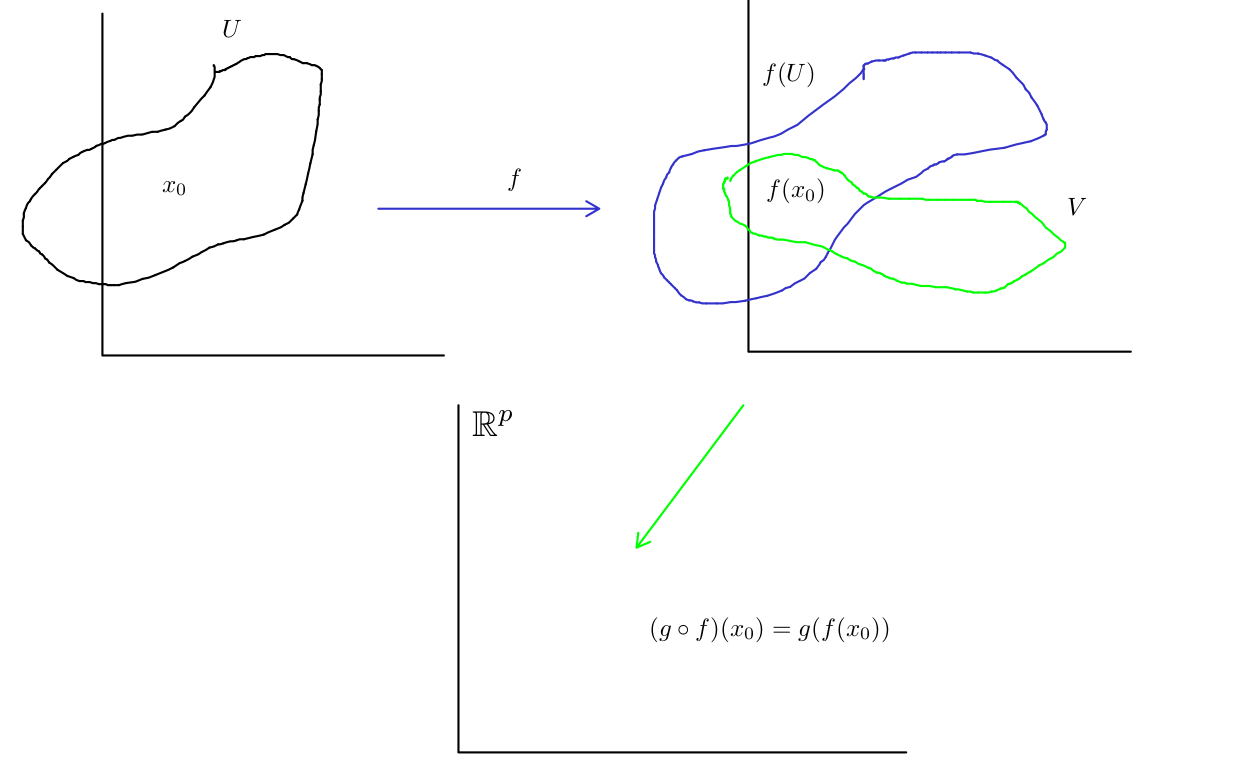
\includegraphics[scale=0.3]{figures/composition.png}
  \caption{La différentiation composée}
  \label{}
\end{figure}

Si $f$ est continue, $g \circ f$ est définie dans un voisinage de $x_0$, par exemple dans une boule ouverte $B(x_0, r) = \tilde{U} \subset U \cap f ^{-1} (V)$.

$g \circ f : \tilde{U} \to \mathbb{R}^p$.

Supposons que les trois dérivées $Df(x_0), Dg(f(x_0)), D(g \circ f)(x_0)$ existent.

$Df(x_0) \in \mathscr{L}(\mathbb{R}^n, \mathbb{R}^m) $.

$D(g(f(x_0))) \in \mathscr{L}(\mathbb{R}^m, \mathbb{R}^p) $.

$D(g \circ f) \in (\mathbb{R}^n, \mathbb{R}^p)$.

\begin{thm}
  Supposons que $f$ est dérivable en $x_0 \in U$ avec la dérivée $Df(x_0)$ et $g$ est dérivable en $f(x_0) \in V$ avec la dérivée $Dg(f(x_0))$, alors $g \circ f$ est bien dérivable en $x_0 \in U$ et

  $$ D(g \circ f)(x_0) = Dg(f(x_0)) \circ Df(x_0).$$
\end{thm}

Si on utilise les matrices jacobiennes de chaque dérivée ($1 \leq k \leq m, 1 \leq j \leq n, 1 \leq i \leq p$),

\begin{gather*}
  \left[ \frac{\partial (g \circ f)_i }{\partial x_j}  \right]_{p \times n}(x_0) = \left[ \frac{\partial g_i }{\partial y_k }  \right] _{p \times m}(f(x_0))  \times \left[ \frac{\partial f_k }{\partial x_j} \right] _{m \times n}(x_0).
\end{gather*}

\begin{gather*}
  \left[ \frac{\partial z_i }{\partial x_j } \right](x_0) = \left[ \frac{\partial z_i }{\partial y_k } \right](f(x_0)) \times \left[\frac{\partial y_k }{\partial x_j} \right](x_0).
\end{gather*}

On a :

$$ \frac{\partial z_i }{\partial x_j } (x_0) = \sum_{k=1}^{n} \frac{\partial z_i }{\partial y_k}  (f(x_0)) \frac{\partial y_k }{\partial x_j} (x_0). $$

$f : U \to \mathbb{R}^m, U \subseteq \mathbb{R}^n$, $V = f(U)$ est ouvert et $g : V \to \mathbb{R}^n$ est l'inverse de $f$.

Donc $g \circ f : U \to \mathbb{R}^n$ et $g \circ f = \mathds{1} _{U}$.

Si en plus $f$ et $g$ sont différentiables, alors $m=n$ et $\forall x \in U, Dg(f(x)) = (Df(x)) ^{-1} $, c'est à dire en particulier $Df(x)$ est une transformation linéaire inversible.

\begin{proof}
  Si $f$ est dérivable en $x \in U$ et $g$ dérivable en $f(x) \in V$,  $\mathds{1} = g \circ f$ dérivable en $x_0$ et

  $$ D \mathds{1} _{U}(x_0) = D(g(f(x_0))) \circ Df(x_0).$$

  $$ \mathds{1} _{U}(x) = x \implies D \mathds{1} _{U}(x_0) \in \mathscr{L}(\mathbb{R}^n, \mathbb{R}^n).$$

  Donc  $$ \mathds{1} _{\mathbb{R}^n} = Dg(f(x_0)) \circ Df(x_0).$$

  Ainsi comme $g$ est linéaire de $f$ on a $f \circ g = \mathds{1} _{V}$, donc

  $$ \mathds{1} _{\mathbb{R}^m} = Df(x_0) \circ Dg(f(x_0)).$$
\end{proof}

\begin{lemma}
  Si $L : \mathbb{R}^n \to \mathbb{R}^m$ est une fonction linéaire, $\overrightarrow{ b } \in \mathbb{R}^m $ et $T(x) = L(x) + \overrightarrow{ b } $, $T : \mathbb{R}^n \to \mathbb{R}^m$.

  Ainsi $T$ est différentiable dans $\mathbb{R}^n$ et

  $$ \forall x \in \mathbb{R}^n, DT(x) = L.$$
\end{lemma}

Dans ce cas, $DT : \mathbb{R}^n \to \mathscr{L}(\mathbb{R}^n, \mathbb{R}^m) $ est une application constante (les dérivées partielles de $T$ aussi).

\section{Inversion locale, fonctions implicites, théorème du rang}


\begin{thm}[de Bronner]
  Si $U \subseteq \mathbb{R}^n, V \subseteq \mathbb{R}^m$, $h : U \to V$ est un homéomorphisme (i. e. $h$ continue, inversible et d'inverse \textbf{continue} $h ^{-1} : V \to U$), alors $m=n$.
\end{thm}

\subsection{Théorème de l'application inverse}


\begin{thm}[De l'application inverse]
  $U \subseteq \mathbb{R}^n, x_0 \in U, f : U \to \mathbb{R}^{n}$, $f$ est de classe $\mathcal{C}^1$. Supposons que $Df(x_0) \in \mathscr{L}(\mathbb{R}^n, \mathbb{R}^n) $ est inversible.

  Alors il existe des ensembles ouverts $W \subset U$, $x_0 \in W$ et $V \subseteq \mathbb{R}^n$ tels que $f _{|W} : W \to V$ est inversible. L'inverse $(f _{|W}) ^{-1} : V \to W$ est aussi de classe $\mathcal{C}^1$.
\end{thm}

\begin{figure}[h!]
  \centering
  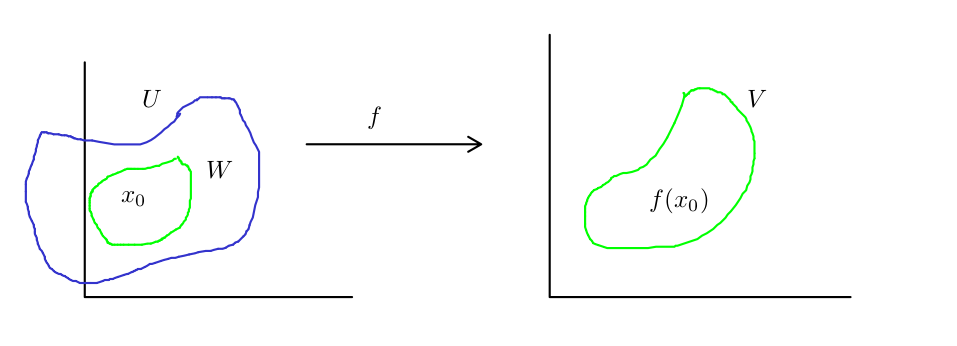
\includegraphics[scale=0.3]{figures/fct_inv.png}
  \caption{Fonctions inversibles}
  \label{}
\end{figure}

\begin{remark}
  Si en plus $f$ est de classe $\mathcal{C}^r$, alors $(f _{|W}) ^{-1} $ est aussi de classe $\mathcal{C}^r$.
\end{remark}

Notons que $\forall y \in V, x \in W, f(x)=y$,

\begin{gather*}
  (D(f _{|W})^{-1} )(y) = (Df(x)) ^{-1}.
\end{gather*}

En particulier, il existe $W$ tel que $Df(x)$ est inversible pour tout $x \in W$.

\subsection{Théorème du rang}


\marginpar{20-09-2023}

\begin{thm}[Du rang]
  $f : U \to \mathbb{R}^m$, $U \subset \mathbb{R}^n$ de classe $\mathcal{C}^r, r \geq 1$.  Supposons que $\forall x \in U$,

  \[
  \operatorname{rang}(Df(x)) \equiv k,
  \]

  où $1 \leq k \leq m$ est fixé.

  $(Df(x) : \mathbb{R}^n \to \mathbb{R}^m, \text{ donc } 0 \leq \operatorname{rang}(Df(x)) \leq m)$.

  Soit $x_0 \in U$. Alors il y a des ouverts $W \subseteq \mathbb{R}^n, V \subseteq \mathbb{R}^m, x_0 \in W, f(x) \in V$, 2 applications de classe $\mathcal{C}^r$ inversibles

\[
\begin{matrix}
  \varphi : W \to W', \varphi(x_0) =0, W' \subseteq \mathbb{R}^n \\
  \psi : V \to V', \psi(f(x_0)) = 0, V' \subseteq \mathbb{R}^m
\end{matrix}
\]
 telles que $\forall z \in W', z=(z_1, \dots, z_n)$,

  \[
  \psi \circ f \circ \varphi ^{-1} (z_1,z_2, \dots, z_n) = (z_1, z_2, \dots, z_k, 0, \dots, 0).
  \]
\end{thm}

\begin{figure}[h!]
  \centering
  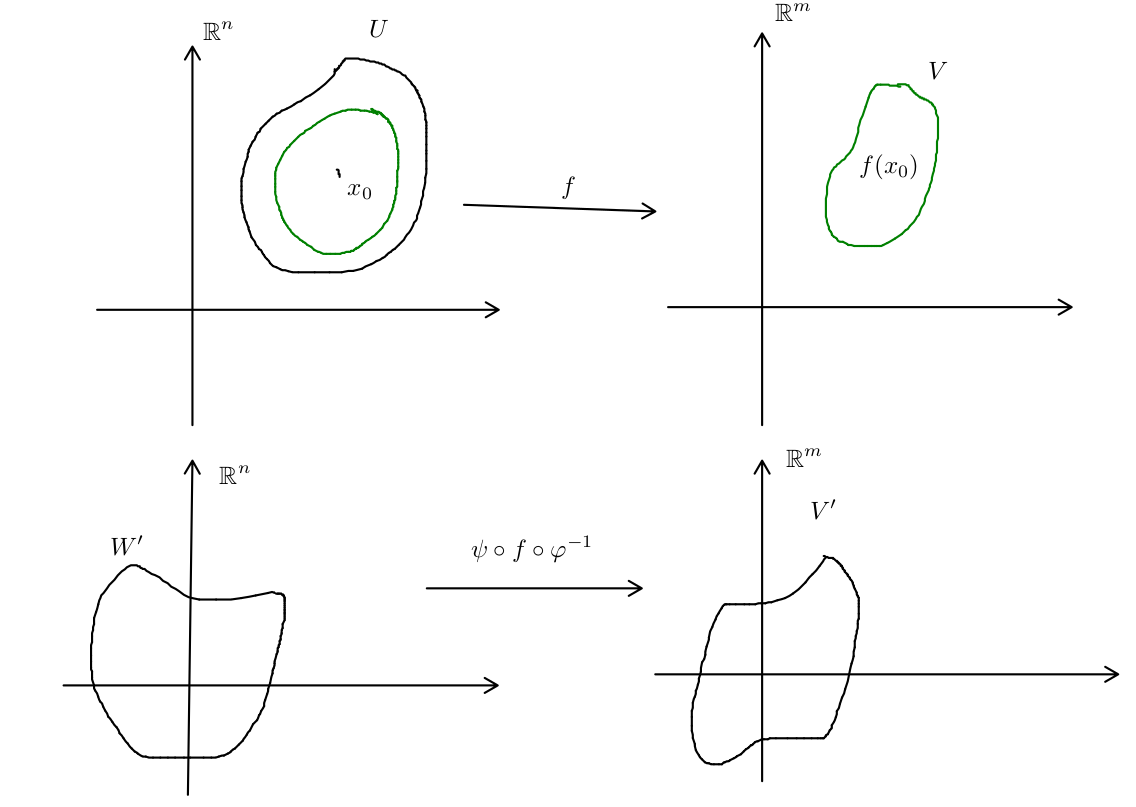
\includegraphics[scale=0.3]{figures/thm-rang.png}
  \caption{Illustration du théorème de rang}
  \label{}
\end{figure}

En particulier, $f(W)$ est un objet de dimension $k$, de régularité $\mathcal{C}^r$ (Si $m=3, k=2, f(W)$ est une surface de classe $\mathcal{C}^r$) et pour tout $y \in f(W), f ^{-1} (y)$ est un objet de dimension $n-k$ de régularité $\mathcal{C}^r$.

On note que les deux applications $\varphi$ et $\psi$ sont de classe $\mathcal{C}^r$ et inversibles. On peut démontrer que dans ce cas-là, les inverses $\varphi ^{-1} $ et $\psi ^{-1} $ sont aussi de classe $\mathcal{C}^r$.

\[
D \varphi ^{-1} (y) = (D \varphi (\varphi ^{-1} (y))^{-1} ), y \in W'.
\]

$\varphi ^{-1} $ étant continue, $D \varphi$ étant continue, l'inverse d'une matrice étant continue tant que $\operatorname{det} \neq 0$, $\varphi$ est de classe $\mathcal{C}^1$ inversible $\implies \varphi ^{-1} $ est de classe $\mathcal{C}^1$.

\begin{definition}[Difféomorphisme]
  Soient $U, U' \subseteq \mathbb{R}^n$ ouverts.

  Si $\varphi : U \to U'$ est une application de classe $\mathcal{C}^r$, avec l'inverse $\varphi ^{-1} : U' \to U$ de classe $\mathcal{C}^r$, on dit que $\varphi$ est un difféomorphisme de classe $\mathcal{C}^r$.
\end{definition}

\begin{remark}[Le théorème de rang dans le cas spécial où $f$ est linéaire]
  Soit $L : \mathbb{R}^n \to \mathbb{R}^m$, $\operatorname{rang}(L) = k, 0 \leq k \leq m$, alors il existe deux bases $\alpha_n$ et $\beta_m$ pour $\mathbb{R}^n$ et $\mathbb{R}^m$ telles que

  \[
  [L] _{\alpha_n} ^{\beta_m} =  \left[\begin{matrix}
    1 & 0 & \dots & 0 \\
    0 & 1 & \dots & 0 \\
    \vdots & \vdots & \ddots & \vdots \\
    0 & 0 & \dots & 0
  \end{matrix}\right] _{m \times n}.
  \]

  (En exercice).
\end{remark}

\begin{corollary}\label{inj}
  $U \subseteq \mathbb{R}^n, f : U \to \mathbb{R}^m$, $f$ est $\mathcal{C}^r, r \geq 1$.

  Supposons que pour $x_0 \in U$, $Df(x_0)$ est injective. $Df(x_0) \in \mathscr{L}(\mathbb{R}^n, \mathbb{R}^m) $. Alors il existe un voisinage $W$ de $x_0$ tel que $f$ est injective sur $W$.
\end{corollary}

Pour $x \in U,$

\[
Df(x) = \left[\begin{matrix}
  \frac{\partial f }{\partial x_1} & \dots & \frac{\partial f }{\partial x_n }
\end{matrix}\right] _{m \times n}.
\]

Si $Df(x_0)$ est injective, $\operatorname{rang}(Df(x_0)) = n \ (m \geq  n)$. On obtient une sous-matrice de $Df(x)$ de taille $n \times n$ inversible.

\begin{lemma}[D'algèbre linéaire]
  $A \in \mathbb{R} ^{m \times n}$. Alors $\operatorname{rang} A = n$ si et seulement si il existe une sous-matrice $B \in \mathbb{R} ^{n \times n}$ de $A$ telle que $\operatorname{det} B \neq 0$.

  %\[
  %\left[\begin{matrix}
  %  \overrightarrow{ v_1 } & \dots & \overrightarrow{ v_n }
  %\end{matrix}\right],
  %\]

  %$\overrightarrow{ v_j } \in \mathbb{R}^m $.

  (En exercice).
\end{lemma}

Alors sous les hypothèse du corollaire \ref{inj}, $\operatorname{rang}Df(x) \equiv n$ dans un voisinage $W$ de $x_0$, appliquant le théorème du rang

\[
\tilde{f} = \varphi \circ f \circ \varphi ^{-1} (z_1, \dots, z_n) = (z_1, \dots, z_n, 0, \dots, 0)
\]

qui est injectif.

\begin{corollary}
  Les mêmes hypothèses que dans le corollaire \ref{inj}.

  Si $Df(x_0)$ est surjective, alors il existe un voisinage ouvert $V \subseteq f(U)$ de $f(x_0)$ (c'est à dire $f(x_0)$ est un point intérieur de $f(U))$ tel que $f$ est surjective sur $V$.
\end{corollary}

Argument à travers l'observation de l'algèbre linéaire qui dit que si $\operatorname{rang}(A) = m, m \leq n, A \in \mathbb{R}^{m \times n}$, il  y a une sous-matrice $B \in \mathbb{R}^{m\times m}$ tel que $\operatorname{det}(B) \neq 0$.

Théorème de rang : $k=m \leq n$.

Les détails en exercice.

\subsection{Théorème de fonctions implicites}


\begin{thm}[De fonctions implicites]
  $U \subseteq \mathbb{R}^n, V \subseteq \mathbb{R}^m$, $F : U \times V \to \mathbb{R}^m$ une application $\mathcal{C}^r, r \geq 1$.

  $(x_0, y_0) \in U \to V$ donné.

  \[
  DF(x_0) \in \mathbb{R}^{m \times (m+n)}
  \]

  et

  \[
  DF(x_0) = \left[\begin{matrix}
    \frac{\partial F }{\partial x_1} & \dots &\frac{\partial F }{\partial x_n } & \mid & \frac{\partial F }{\partial y_1 } & \dots & \frac{\partial F }{\partial y_m }
  \end{matrix}\right] _{m \times (m+n)}.
  \]

  Pour tout $(x_0, y_0) \in U \times V, DyF(x_0, y_0) \in \mathbb{R}^{m \times m}$. Supposons que $DyF(x_0)$ est inversible. Alors il existe un voisinage $W$ de $x_0$ dans $U$ et une application $\mathcal{C}^r$ $f : W \to V$ telle que $f(x_0) = y_0$ et

  \[
  \forall x \in W, F(x, f(x)) = F(x_0, y_0).
  \]
\end{thm}

\begin{figure}[h!]
  \centering
  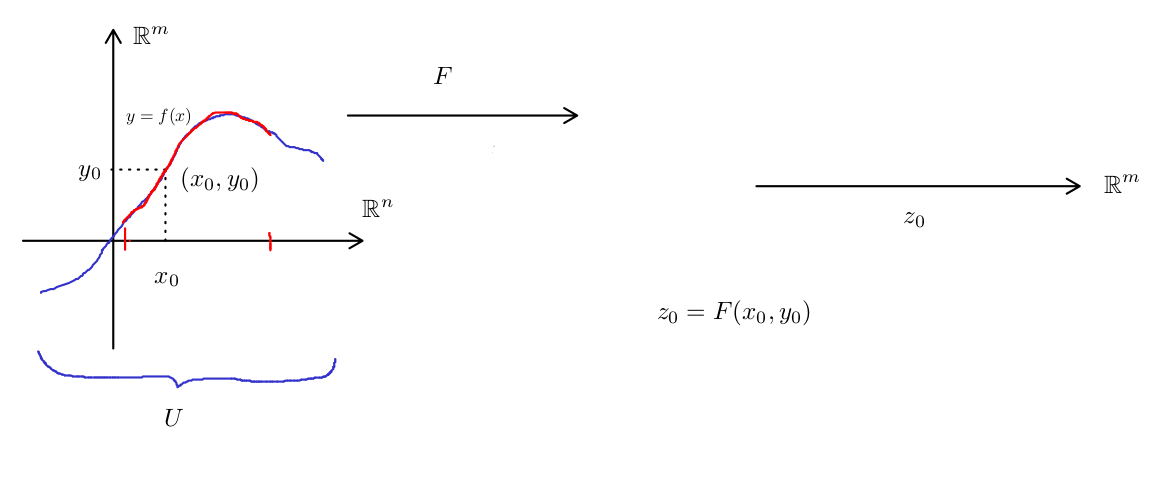
\includegraphics[scale=0.3]{figures/fct_impl.png}
  \caption{Illustration du théorème de fonctions implicites}
  \label{}
\end{figure}

Donc le graphe de $x \longrightarrow f(x)$ dans $W \times V$ pour l'application $f: W \to V$ est à l'intérieur de $F ^{-1} (x_0)$.

On peut dire que la fonction implicite

\[
F(x,y) = z_0, x \in \mathbb{R}^n, y \in \mathbb{R}^m, z_0 \in \mathbb{R}^n
\]

peut être exprimée explicitement $y = f(x)$ dans un voisinage $W$.

\paragraph{Exemple}

$m=1=n$.

Si $F(x, y) = y ^2-x$.

\subparagraph{Exemple 1} $x_0 = 0, y_0 =1 , z_0 =1$.

\[
DF = \left[\begin{matrix}
  \frac{\partial F }{\partial x} & \frac{\partial F }{\partial y }
\end{matrix}\right] = \left[\begin{matrix}
  -1 & 2y
\end{matrix}\right] \in \mathcal{C}^\infty.
\]

\[
DyF = [2y] _{|x|}.
\]

\[
DyF(x_0, y_0) = 2 y_0 = 2 \neq 0.
\]

Donc près de $(0, 1) = (x_0, y_0), y= f(x)$ a une solution $\mathcal{C} ^{\infty}$.

Mais si $x_0 = 0, y_0 = 0, z_0 = 0$, $DyF(x_0, y_0)=2y_0=0$ n'est pas inversible. $F$ est $\mathcal{C}^\infty$.

Implicitement, près de $(0, 0)$, on a $y ^2 - x = 0$.

On essaie de trouver $y=f(x)$.

$y ^2 = x \implies y = \pm \sqrt{ x } $.

Mais $\sqrt{\cdot} $ n'est pas définie pour $x \less 0$ près de $x_0 = 0$!

Donc il n'y a pas un moyen d'écrire explicitement $F(x,y) = 0$ près de $(0, 0)$ comme une fonction $\mathcal{C}^\infty$.

\begin{remark}[Sur le théorème des fonctions implicites]
  En effet, si $W' = f(W) \subset V$, on a

  \[
  (x,y) \in W \times W', F(x,y) = z_0 \iff y=f(x).
  \]
\end{remark}

\section{Algèbre multilinéaire}

Soit $E$ espace vectoriel sur $\mathbb{R}$ de dimension finie $n$, c'est-à-dire il existe $\beta = \{ \overrightarrow{ v_1 }, \dots, \overrightarrow{ v_n }   \} $ base telle que

\[
\forall \overrightarrow{ v } \in E, \exists ! (\alpha_1, \dots, \alpha_n), \overrightarrow{ v } = \sum_{i=1}^{n} \alpha_i \overrightarrow{ v_i }.
\]

En particulier, $\beta $ engendre $E$ ($E = \operatorname{span}(\beta) = \langle \beta \rangle $) si $\beta$ est libre.

\subsection{L'espace dual $E ^{*}$}

\[
E ^{*} = \{ T : E \to \mathbb{R} \text{ linéaire}  \} = \mathscr{L}(E, \mathbb{R}) .
\]


\begin{thm}
  On a $\operatorname{dim}(E ^{*}) = \operatorname{dim}(E)$.
\end{thm}

\begin{proof}
  Supposons $\beta = (e_1, \dots, e_n) $ est une base ordonnée de $E$. On définit alors $n$ éléments $(e ^{1}, e ^2, \dots, e ^{n})$, $e ^{j} \in E ^{*}$ de la manière suivante :

  \[
  e ^{j}(e_i) = \delta _{i} ^{j} = \begin{cases}
    1 \text{ si } i=j \\
    0 \text{ sinon. }
  \end{cases}
  \]

  \begin{remark}[Personnelle]
    $e ^{j}$ est l'évaluation du vecteur $\overrightarrow{ v } \in E$ en $e_j$.
  \end{remark}

  Donc $\displaystyle e ^j \left(\sum_{i=1}^{n} \alpha_i e_i \right) = \sum_{i=1}^{n} \alpha_i e ^{j}(e_i) = \sum_{i=1}^{n} \alpha_i \delta _{i} ^{j} = \alpha_i   $.

  Donc $\forall j \in \{ 1, \dots, n \}, e ^{j} \in E ^{*} $, $\beta ^{*} = \{ e ^{1}, \dots, e ^{n} \} $. On montre que $\beta ^{*}$ est une base pour $E ^{*}$.

  \begin{enumerate}
    \item $\beta ^{*}$ est libre. Supposons que pour $c_j \in \mathbb{R}$,

    \[
    \sum_{j=1}^{n} c_j e ^{j} = 0 \in E ^{*}.
    \]



    Donc pour tout $i$,
    \begin{gather*}
      \left(\sum_{j=1}^{n} c_j e ^{j} \right) (e_i) = 0 \in \mathbb{R} \text{ et } \\
      \left(\sum_{j=1}^{n} c_j e ^{j} \right) (e_i) = \sum_{j=1}^{n}c_j e ^{j}(e_i) = \sum_{j=1}^{n}c_j \delta_i ^{j} = c_i.
    \end{gather*}

    Donc $\forall i, c_i = 0$.

    \item $\beta ^{*}$ engendre $E ^{*}$. Soit $T \in E ^{*}$. Est-ce qu'il existe $\alpha_1,\dots, \alpha_n$ tel que

    \[
    T = \sum_{j=1}^{n} \alpha_j e ^{j} \ ?
    \]

    Essayons de trouver les $\alpha_j$ en appliquant l'identité desirée en $e_i$.

    \begin{gather*}
      \forall i, T(e_i) = \left( \sum_{j=1}^{n} \alpha_j e_j \right)(e_i) = \sum_{j=1}^{n} \alpha_j e_j(e_i) = \sum_{j=1}^{n} \alpha_j \delta_i ^{j} = \alpha_i.
    \end{gather*}

    Donc pour $T \in E ^{*}$ donnée, le candidat pour $\alpha_i$ est

    \[
    \forall i \in \{ 1, \dots, n \}, \alpha_i \in T(e_i) \in \mathbb{R},
    \]

    et on obtient que

    \[
    \forall i \in \{ 1, \dots, n \}, T(e_i) = \left(\sum_{j=1}^{n} \alpha_j e ^{j} \right) (e_i).
    \]

    Comme $T$ et $\tilde{T}$ ont les mêmes valeurs sur la base $\beta $, donc $T = \tilde{T}$.

    \[
    T = \sum_{j=1}^{n} T(e_j) e ^{j}.
    \]

  \end{enumerate}
\end{proof}


\begin{definition}
  On dit que $\beta ^{*}$ est la base duale de $\beta $.
\end{definition}

On considère le dual du dual $E ^{**} = (E ^{*}) ^{*}$.


\begin{thm}
  Si $\operatorname{dim}(E) \less \infty$, il y a un isomorphisme canonique entre $E$ et $E ^{**}$.
\end{thm}

On peut définir $E \to E ^{**}$. On pose $e : E \to E ^{**}$.

\[
(\iota(\overrightarrow{ v } ))(T) = T(\overrightarrow{ v } ),
\]

$\forall T \in E ^{*} = \mathscr{L}(E, \mathbb{R}) $.

\begin{exo}

  \

  \begin{enumerate}
    \item Montrer que $\forall v \in E, \iota(\overrightarrow{ v } ) : E ^{*} \to \mathbb{R}$ est une transformation linéaire.
    \item Montrer que $\iota : E \to E ^{**}$ est une transformation linéaire.
    \item Montrer que $\iota$ est bijective (donc un isomorphisme).
  \end{enumerate}
\end{exo}

\begin{proof}

  \

  \begin{enumerate}
    \item \begin{gather*}
      \iota(\overrightarrow{ v } ) (\alpha T+ S) = (\alpha T+S)(\overrightarrow{ v } ) = \alpha T(\overrightarrow{ v } )+ S(\overrightarrow{ v } ) = \alpha \iota(\overrightarrow{ v } )(T)+ \iota(\overrightarrow{ v } )(S).
  \end{gather*}
    \item $\iota : E \to E ^{**}$ est linéaire.

    \begin{gather*}
      \iota(\alpha \overrightarrow{ v } + \overrightarrow{ w }  )(T) = T(\alpha \overrightarrow{ v } + \overrightarrow{ w } ) \stackrel{T \text{ linéaire} }{=} \alpha T(\overrightarrow{ v } )+ T(\overrightarrow{ w } ) \\
      = \alpha \iota(\overrightarrow{ v } )(T)+ \iota(\overrightarrow{ w } ) (T) = \alpha \iota (\overrightarrow{ v } )+ \iota(\overrightarrow{ w }).
    \end{gather*}

    Comme c'est vrai $\forall T \in E ^{*}$, on a l'identification $\iota(\alpha \overrightarrow{ v }+ \overrightarrow{ w }  ) = \alpha \iota(\overrightarrow{ v } )+ \iota(\overrightarrow{ w } )$ (comme un élément de $E ^{**}$). Donc $\iota$ est une transformation linéaire.

    \item On sait que $dim E = dim E ^{*} = dim E ^{**}$ (ce qui veut dire que $\iota$ est surjective). Pour démontrer que $\iota$ est un isomorphisme, il suffit de démontrer que $\operatorname{Ker}(\iota) = \{ 0 \} $ (que $\iota$ est injective).

    Si $\overrightarrow{ v }  \in \operatorname{Ker}(\iota)$, alors $\iota(\overrightarrow{ v } ) = 0 \implies \forall T \in E ^{*}, T(\overrightarrow{ v } ) = \iota(\overrightarrow{ v })(T) = 0(T) =0$, donc $\overrightarrow{ v } $ est tel que $\forall T \in E ^{*}, T(\overrightarrow{ v } ) =0$.

    Si $\overrightarrow{ v } \neq \overrightarrow{ 0 }  $, on peut compléter $\overrightarrow{ v } $ avec une base $\{ \overrightarrow{ v }, \overrightarrow{ v_2 },\dots, \overrightarrow{ v_n } \} $ de $E$ et définir $T(\alpha_1 \overrightarrow{ v } + \alpha_2 \overrightarrow{ v_2 } + \dots + \alpha_n \overrightarrow{ v_n }  ) = \alpha_1$. Dans ce cas-là, $T(\overrightarrow{ v } ) = 1 \neq 0$.

    Si $\beta = (e_1, \dots, e_n)$ base de $E$. On a vu que la base duale $\beta ^{*} = (e ^{1}, e ^2, \dots, e ^{n})$ est une base de $E ^{*}$.

    \[
    e ^{j}(e_i) = \delta_i ^{j}.
    \]

    \[
    (\beta ^{*}) ^{*} = \beta ^{**} = (\eta_1, \eta_2, \dots, \eta_n).
    \]

    \begin{equation} \label{base1}
      \forall i, \eta_i \in E ^{**}, \eta_i(e ^{i}) = \delta_i ^{j}, \forall i, j.
    \end{equation}

    On va aussi calculer

    \begin{equation} \label{base2}
      \iota(e_i)(e ^{j}) = e ^{j}(e_i) = \delta_i ^{j}.
    \end{equation}

    $\forall e ^{j}$ de base $\beta ^{*}$, on a

    \[
    \eta_i(e ^{j}) = \iota(e_i)(e ^{j}), \eta_i, \iota(e_i) \in E ^{**} = \mathscr{L}(E ^{*}, \mathbb{R}).
    \]

    $\eta _i$ et $i(e_i)$ coincident sur une base de $E ^{*}$, donc

    \[
    \forall i, \eta_i = \iota(e_i).
    \]

    Pour simplifier, parfois on identifie $E$ et $E ^{**}$ par l'application $\iota$, c'est-à-dire on met $\overrightarrow{ v } = \iota(\overrightarrow{ v })$.
  \end{enumerate}
\end{proof}

Les éléments de $E ^{*}$ sont appelés \textbf{les vecteurs covariants}. Les éléments de $E ^{**}$ sont appelés \textbf{les vecteurs contravariants}.

\subsection{Les applications multilinéaires}

Supposons que $E_1, E_2, \dots, E_k$ sont des espaces vectoriels sur $\mathbb{R}$ et $E'$ espace vectoriel de $\mathbb{R}$.

\[
\alpha : E_1 \times E_2 \times \dots \times E_k \longrightarrow E'
\]

est une application $k$-linéaire quand $\alpha$ est linéaire par rapport à chaque coordonnée dans l'un des espaces $E_j$ quand les autres coordonnées (composantes) sont fixées.

$\overrightarrow{ v_i } \in E_i $, $1 \leq i \leq k$, $\alpha(\overrightarrow{ v_1 }, \overrightarrow{ v_2 }, \dots, \overrightarrow{ v_k })$.

Si $\forall i \in \{ 1, \dots, k \}$, $a \in \mathbb{R}, \forall \overrightarrow{ v_j } \in E_j, \overrightarrow{ w } \in E_i $, on a

\[
\alpha(\overrightarrow{ v_1 }, \overrightarrow{ v_2 }, \dots, a \overrightarrow{ v_i }+ \overrightarrow{ w }, \dots, \overrightarrow{ v_k }) = a \alpha(\overrightarrow{ v_1 }, \dots, \overrightarrow{ v_i }, \dots, \overrightarrow{ v_k })+ \alpha(\overrightarrow{ v_1 }, \overrightarrow{ v_2 }, \dots, \overbrace{\overrightarrow{ w } }^{i\text{-ème}}, \dots, \overrightarrow{ v_k }).
\]

\paragraph{Exemple}

\begin{enumerate}
  \item $f(x,y) = xy$, $f : \stackrel{E_1}{\mathbb{R}} \times \stackrel{E_2}{\mathbb{R}} \to \stackrel{E'}{\mathbb{R}}$.
  \item $E_1 = E_2 = \mathbb{R}^n$, $E' = \mathbb{R}$,

  \[
  \alpha(\overrightarrow{ v_1 }, \overrightarrow{ v_2 } ) = \overrightarrow{ v_1 }\cdot \overrightarrow{ v_2 } \text{ 2-linéaire. }
  \]

  \item $E_1 = E_2 = E_3 \equiv \mathbb{R}^3$, $E' = \mathbb{R}$.
  \[
  \alpha(\overrightarrow{ v_1 }, \overrightarrow{ v_2 }, \overrightarrow{ v_3 }) = \overrightarrow{ v_1 } \cdot (\overrightarrow{ v_2 } \wedge \overrightarrow{ v_3 }  ) = det \left( \left[\begin{matrix}
  \overrightarrow{ v_1 } \\
  \overrightarrow{ v_2 }  \\
  \overrightarrow{ v_3 }
  \end{matrix}\right]\right)  _{3 \times 3}.
  \]

  Cette application est 3-linéaire.

  \item $E_1 = E_2 = \dots = E_n = \mathbb{R}^n$.

  \[
  \alpha(\overrightarrow{ v_1 }, \overrightarrow{ v_2 }, \dots, \overrightarrow{ v_n } ) = det \left(\left[\begin{matrix}
  \overrightarrow{ v_1 } \\
  \overrightarrow{ v_2 } \\
  \vdots \\
  \overrightarrow{ v_n }
  \end{matrix}\right]\right).
  \]

  C'est une application $n$-linéaire.

  \item Le déterminant d'une matrice de taille $n \times n$ est une application $n$-linéaire.
\end{enumerate}




\subsubsection{Quelques notations}

$E$ espace vectoriel de dimension finie.

On note $\Omega ^{k}(E) := \{ \alpha : \underbrace{E \times E \times \dots \times E}_{k \text{ fois} }  \to \mathbb{R} \mid \alpha \text{ est } k \text{-linéaire}  \} $.

Remarquons que $\Omega ^{1}(E) = \{ \alpha : E \to \mathbb{R} \mid \alpha \text{ est linéaire}  \} = E ^{*}$.

\begin{prop}
  $\forall k \in \mathbb{N} ^{*}, \Omega ^{k}(E) $ est un espace vectoriel de dimension $n ^{k}$.
\end{prop}

\begin{proof}
  Si $\alpha, \beta \in \Omega ^{k}(E), a \in \mathbb{R}$. Il faut démontrer que $a \alpha+ \beta$ est aussi une application $k$-linéaire sur $E ^k = \overbrace{E \times \dots \times E}^{k \text{ fois}}$.

  \begin{gather*}
    a \alpha + \beta (b \overrightarrow{ v_1 }+ \overrightarrow{ w }, \dots) = a[\alpha(b \overrightarrow{ v_1 }+ \overrightarrow{ w }, \dots)]+ \beta(b \overrightarrow{ v_1 }+\overrightarrow{ w })\\
    = a[b \alpha(\overrightarrow{ v_1 }, \dots)+ \alpha(\overrightarrow{ w }, \dots)] + b \beta(v_1, \dots) + \beta(\overrightarrow{ w }, \dots) \\
    = b[a \alpha+ \beta](\overrightarrow{ v_1 }, \dots )+ [a \alpha+ \beta](\overrightarrow{ w }, \dots)
  \end{gather*}

  De même pour chaque $1 \leq i \leq k$.

  Pour trouver la dimension de $\Omega ^{k}(E)$, il faudra trouver une base de $\Omega ^{k}(E)$. Pour cela, il faudra d'abord introduire ``le produit tensoriel''.
\end{proof}

\begin{definition}[Produit tensoriel]
  Supposons que $\alpha : E_1 \times \dots \times E_k \to \mathbb{R}$ $k$-linéaire, $\beta: E_1' \times \dots \times E_l' \to \mathbb{R}$ $l$-linéaire.

  On définit

  \[
  \alpha \otimes \beta : E_1 \times \dots \times E_k \times E_1' \times \dots \times E_l' \longrightarrow \mathbb{R}
  \]

  telle que

  \[
  \alpha \otimes \beta(\overrightarrow{ v_1 }, \dots, \overrightarrow{ v_k }, \overrightarrow{ v_1' }, \dots, \overrightarrow{ v_l'} ):=\alpha(\overrightarrow{ v_1 }, \dots, \overrightarrow{ v_k }) \beta(\overrightarrow{ v_1' }, \dots, \overrightarrow{ v_l'})
  \]

  qui est une application $(k+l)$-linéaire (avec $\overrightarrow{ v_i } \in E_i, i \in \{ 1, \dots, k \}, \overrightarrow{ v_j' } \in E_j', j \in \{ 1, \dots, l\}$).
\end{definition}

Les applications $k$-linéaires sont appelées les tenseurs covariants d'ordre $k$.

\begin{exo}
  On montre que $\otimes$ est une opération associative.

  $\forall \alpha, \beta, \gamma $ tenseurs covariants,

  \[
  (\alpha \otimes \beta) \otimes \gamma = \alpha \otimes (\beta \otimes \gamma ).
  \]
\end{exo}

\paragraph{Exemple} $E_1 = \mathbb{R}^{n}, E_1' = \mathbb{R} ^{n}, k=l=1, \alpha \in E_1 ^{*}, \alpha(\overrightarrow{ v }) =2 \overrightarrow{ v } \cdot e_1  , \forall \overrightarrow{ v } \in \mathbb{R}^n, \beta \in E_1^{'*}, \beta (\overrightarrow{ v' } ) = \overrightarrow{ v' } \cdot e_1, \forall \overrightarrow{ v' } \in \mathbb{R}^n$.

\[
\alpha \otimes \beta(\overrightarrow{v}, \overrightarrow{ v' }) = 2 (\overrightarrow{ v }\cdot e_1)(\overrightarrow{ v' } \cdot e_1)
\]

et

\[
\beta \otimes \alpha(\overrightarrow{ v' }, \overrightarrow{ v } ) = 2(\overrightarrow{ v' }\cdot e_1 )(\overrightarrow{ v } \cdot e_1 ).
\]

Mais si $\tilde{\beta}(\overrightarrow{ v' } ) = \overrightarrow{ v' } \cdot e_2 $,

\begin{gather*}
  \alpha \otimes \tilde{\beta} (\overrightarrow{ v }, \overrightarrow{ v' }) = 2 (\overrightarrow{ v } \cdot e_1 )(\overrightarrow{ v' }\cdot e_2 ), \\
  \text{mais } \tilde{\beta }\otimes \alpha(\overrightarrow{ v' }, \overrightarrow{ v }  ) = 2 (\overrightarrow{ v' }\cdot e_1 )(\overrightarrow{ v }\cdot e_2 ).
\end{gather*}

Le produit tensoriel n'est donc pas commutatif.

\

$E ^{k} = \underbrace{E \times \dots \times E}_{k \text{ fois} }$

$\Omega ^{k}(E) := \{ \alpha : \underbrace{E \times E \times \dots \times E}_{k \text{ fois} }  \to \mathbb{R} \mid \alpha \text{ est } k \text{-linéaire}  \} $.

\begin{prop}\label{dim-tens}
  $\Omega ^{k}(E)$ est un espace vectoriel de dimension $n ^k$, où $n = dim(E)$.
\end{prop}

\begin{proof}
  $dim E = n$, $(e_1, \dots, e_n)$ est une base de $E$ et $(e ^{1}, \dots, e ^{n})$ est une base de $E ^{*} = \Omega ^{1}(E)$.

  Par exemple si on prend

  \[
  \underbrace{e^{1} \otimes e ^{1} \otimes \dots \otimes e ^{1}}_{k \text{ fois} } : E \times \dots \times E \to \mathbb{R},
  \]

  et

  \begin{gather*}
    e^{1} \otimes e ^{1} \otimes \dots \otimes e ^{1}(\overrightarrow{ v_1 }, \dots, \overrightarrow{ v_n }  ), \overrightarrow{ v_i } \in E, \\
    = e ^{1}(\overrightarrow{ v_1 } ) e ^{1}(\overrightarrow{ v_2 } ) \dots e ^{1}(\overrightarrow{ v_n }).
  \end{gather*}

  $\mathscr{A} = \{ e ^{i_1} \otimes e ^{i_2} \otimes \dots \otimes e ^{i_k} \mid \text{pour } 1 \leq j \leq k, 1 \leq i_k \leq n  \} $.

  Il y a $n$ choix pour chaque $e ^{i_j}$, alors, au total, on a $n ^k$ choix pour les éléments de $\mathscr{A} $, ce qui démontre la proposition \ref{dim-tens}. On montre maintenant que

  \begin{enumerate}
    \item $\mathscr{A} $ engendre $\Omega ^{k}(E)$ ;
    \item $\mathscr{A} $ est libre.
  \end{enumerate}

  Soit $\alpha \in \Omega ^{k}(E)$.

  On va démontrer que

  \[
  \alpha \stackrel{?}{=} \sum_{1 \leq i_1, \dots, i_k \leq n}^{} \alpha(e _{i_1}, e _{i_2}, \dots, e _{i_k}) e ^{i_1} \otimes e ^{i_2} \otimes \dots \otimes e ^{i_k}.
  \]

  Prenons $(\overrightarrow{ v_1 }, \overrightarrow{ v_2 }, \dots, \overrightarrow{ v_n }) \in E ^{k}$. On a

  \begin{gather*}
    \overrightarrow{ v_j } = \sum_{i=1}^{n} c _{ij} e_i.
  \end{gather*}

  \begin{gather*}
    \alpha(\overrightarrow{ v_1 }, \dots, \overrightarrow{ v_k }) = \alpha\left(\sum_{i=1}^{n}c _{i1}e_i, \dots, \sum_{i=1}^{n} c _{ik} e_i\right) \\
    = \sum_{i=1}^{n} c _{i1} \alpha\left(e_i, \sum_{i_2}^{} c _{i_2 2} e _{_2 i}, \dots  \right)  \\
    = \sum_{i_1 =1}^{n} \sum_{i_2=1}^{n} \dots \sum_{i_k=1}^{n} c _{i_1 1} c _{i_2 2} \dots c _{i_k k} \alpha(e _{i_1},\dots, e _{i_k}).
  \end{gather*}

  Maintenant, pour

  \[
  \beta = \sum_{1 \leq i_1, \dots, i_n \leq n}^{} \alpha(e_{i_1}, \dots,  e_{i_n}) e ^{i_1}\otimes \dots \otimes e ^{i_n},
  \]

  on calcule pour $\beta  \in \Omega ^{k}(E)$,

  \begin{gather*}
    \beta (\overrightarrow{ v_1 }, \dots, \overrightarrow{ v_k })= \sum_{i_1}^{} \sum_{i_2}^{} \dots \sum_{i_k}^{} c _{i_1} c _{i_2} \dots c _{i_k} \beta(e _{i_1}, \dots, e _{i_n}).
  \end{gather*}

  Mais

  \begin{gather*}
    \beta (e _{i_1}, \dots, e _{i_k}) = \sum_{1 \leq i_1', \dots, i_k' \leq n}^{} \alpha( e _{i_1'}, e _{i_2'}, \dots, e _{i_k'}) e ^{i_1'}\otimes e ^{i_2'} \otimes \dots \otimes e ^{i_k'} (e_{i_1},\dots, e_{i_k}) \\
    = \sum_{1 \leq i_1' \leq \dots \leq i_k' \leq n}^{} \alpha(e _{i_1'}, \dots, e _{i_k'}) e ^{i_1'}(e _{i_1}) e ^{i_2'}(e _{i_2}) \dots e ^{i_k'} (e _{i_k}) \\
    =\sum_{1 \leq i_1', \dots, i_k' \leq n}^{} \alpha(e _{i_1'}, \dots, e _{i_k'}) \delta _{i_1} ^{i_1'} \dots \delta _{i_k} ^{i_k'} = \alpha(e _{i_1}, \dots, e _{i_n}).
  \end{gather*}

  Donc

  \begin{gather*}
    \beta (\overrightarrow{ v_1 }, \dots, \overrightarrow{ v_k }  ) = \sum_{i_1}^{} \sum_{i_2}^{} \dots \sum_{i_k}^{} c _{i_1 1} c _{i_2 2} \dots c _{i_k k} \alpha(e _{i_1}, \dots, e _{ik}) = \alpha(\overrightarrow{ v_1 }, \dots, \overrightarrow{ v_k }  )   .
  \end{gather*}

  Donc ? est démontré, et on a $\alpha \in span(\mathscr{A} ) = \langle \mathscr{A} \rangle $, où $\mathscr{A} = \{ e ^{i_1} \otimes \dots \otimes e ^{i_k}\} $.

  \

  Montrons que $\mathscr{A} $ est libre. Soit

  \begin{gather*}
    \sum_{1 \leq i_1 , \dots, i_k \leq n}^{} c _{i_1 i_2 \dots i_k}  e ^{i_1} \otimes \dots \otimes e ^{i_k} = 0 \in \Omega ^{k}(E).
  \end{gather*}

  Le même calcul qu'auparavant démontre que

  \[
  0 = 0(e _{i_1}, \dots, e _{i_k}) = c _{i_1 \dots i_k}, \forall i_1, \dots, i_k,
  \]

  donc

  \[
  \forall i_1, \dots, i_k, c _{i_1 \dots i_k} =0,
  \]

  donc $\mathscr{A} $ est libre.
\end{proof}

\begin{remark}
  Si $f : U \to \mathbb{R}^m, U \subseteq \mathbb{R}^n$, $Df(x) \in \mathscr{L}(\mathbb{R}^n, \mathbb{R}^m) $,

  \begin{gather*}
    Df:U \to \mathscr{L}(\mathbb{R}^n, \mathbb{R}^n) \\
    D ^2 f(x) \in \mathscr{L}(\mathbb{R}^n, \mathscr{L}(\mathbb{R}^n, \mathbb{R}^m) ) \\
    \vdots \\
    D ^{n}f(x) \in \mathscr{L}(\mathbb{R}^n, \mathscr{L}(\mathbb{R}^n, \dots, \mathscr{L}(\mathbb{R}^n, \mathbb{R}^m) ) ) .
  \end{gather*}
\end{remark}

\begin{lemma}
  $\mathscr{L}(\mathbb{R}^n, \mathscr{L}(\mathbb{R}^n, \mathbb{R}^m) ) \simeq \{ \alpha : \mathbb{R}^n \times \mathbb{R}^n \to \mathbb{R}^n \mid \alpha \text{ est 2-linéaire} \}  $.
\end{lemma}

Pour un élément $g \in \mathscr{L}(\mathbb{R}^n, \mathscr{L}(\mathbb{R}^n, \mathbb{R}^m) ) $ et $\overrightarrow{ v } \in \mathbb{R}^n, g(\overrightarrow{ v } ) \in \mathscr{L}(\mathbb{R}^n, \mathbb{R}^m) $.

Pour tout $k$, pour tout $x \in U$, $D ^{k}f(x) \in (\Omega ^{k}(\mathbb{R}^n))^{m}$. Cet espace est de dimension $m(n ^{k})$.

On définit

\[
\alpha_g(\overrightarrow{ v } )(\overrightarrow{ w } ) \in \mathbb{R}^n.
\]

On voit que $\alpha _{g}$ est une application 2-linéaire.

Supposons que $\alpha_g = \alpha _{g'}, $ donc $ \forall \overrightarrow{ v }, \overrightarrow{ w } \in \mathbb{R}^n, \alpha _{g}(\overrightarrow{ v }, \overrightarrow{ w }) = \alpha _{g'}(\overrightarrow{ v }, \overrightarrow{ w }) $, donc $g(\overrightarrow{ v } )(\overrightarrow{ w } ) = g'(\overrightarrow{ v } )(\overrightarrow{ w } )$.

Donc $\forall \overrightarrow{ v } \in \mathbb{R}^n, g(\overrightarrow{ v } ) = g'(\overrightarrow{ v } ) \in \mathscr{L}(\mathbb{R}^n, \mathbb{R}^m)$, donc $g = g'$.

On en déduit que $g \longrightarrow \alpha_g$ est injective.





\end{document}
